\documentclass{article}

\author{Tran Van Tan Khoi}

\title{Weekly Homework Report \#2}

\date{April 01, 2025}

\usepackage[T1]{fontenc}
\usepackage[utf8]{inputenc}
\usepackage[a4paper,top=2cm,bottom=2cm,left=3cm,right=3cm,marginparwidth=1.75cm]{geometry}
\usepackage[colorlinks=true, allcolors=blue]{hyperref}
\usepackage{bookmark}
\usepackage{graphicx}


\usepackage{tcolorbox}
\tcbuselibrary{theorems}

\newtcbtheorem[number within=section]{theorem}{}%
{colback=green!5,colframe=green!35!black,fonttitle=\bfseries}{th}

\newtcbtheorem[number within=section]{statement}{Problem}%
{colback=blue!5,colframe=blue!35!black,fonttitle=\bfseries}{th}

\newtcbtheorem[number within=section]{example}{}%
{colback=magenta!5,colframe=magenta!35!black,fonttitle=\bfseries}{th}


\begin{document}
    \maketitle

    \section{Introduction}
    
    This week's set of problems focuses on two basic search techniques: linear search and binary search. Utilizing these techniques masterfully brings tremendous aids in more convoluted algorithm concepts.


    This report, along with C++ solutions, can be found over at \href{https://github.com/xtrkoi/throwaway-rep}{this Github repo}.

    \begin{figure}[!h]
        \centering
        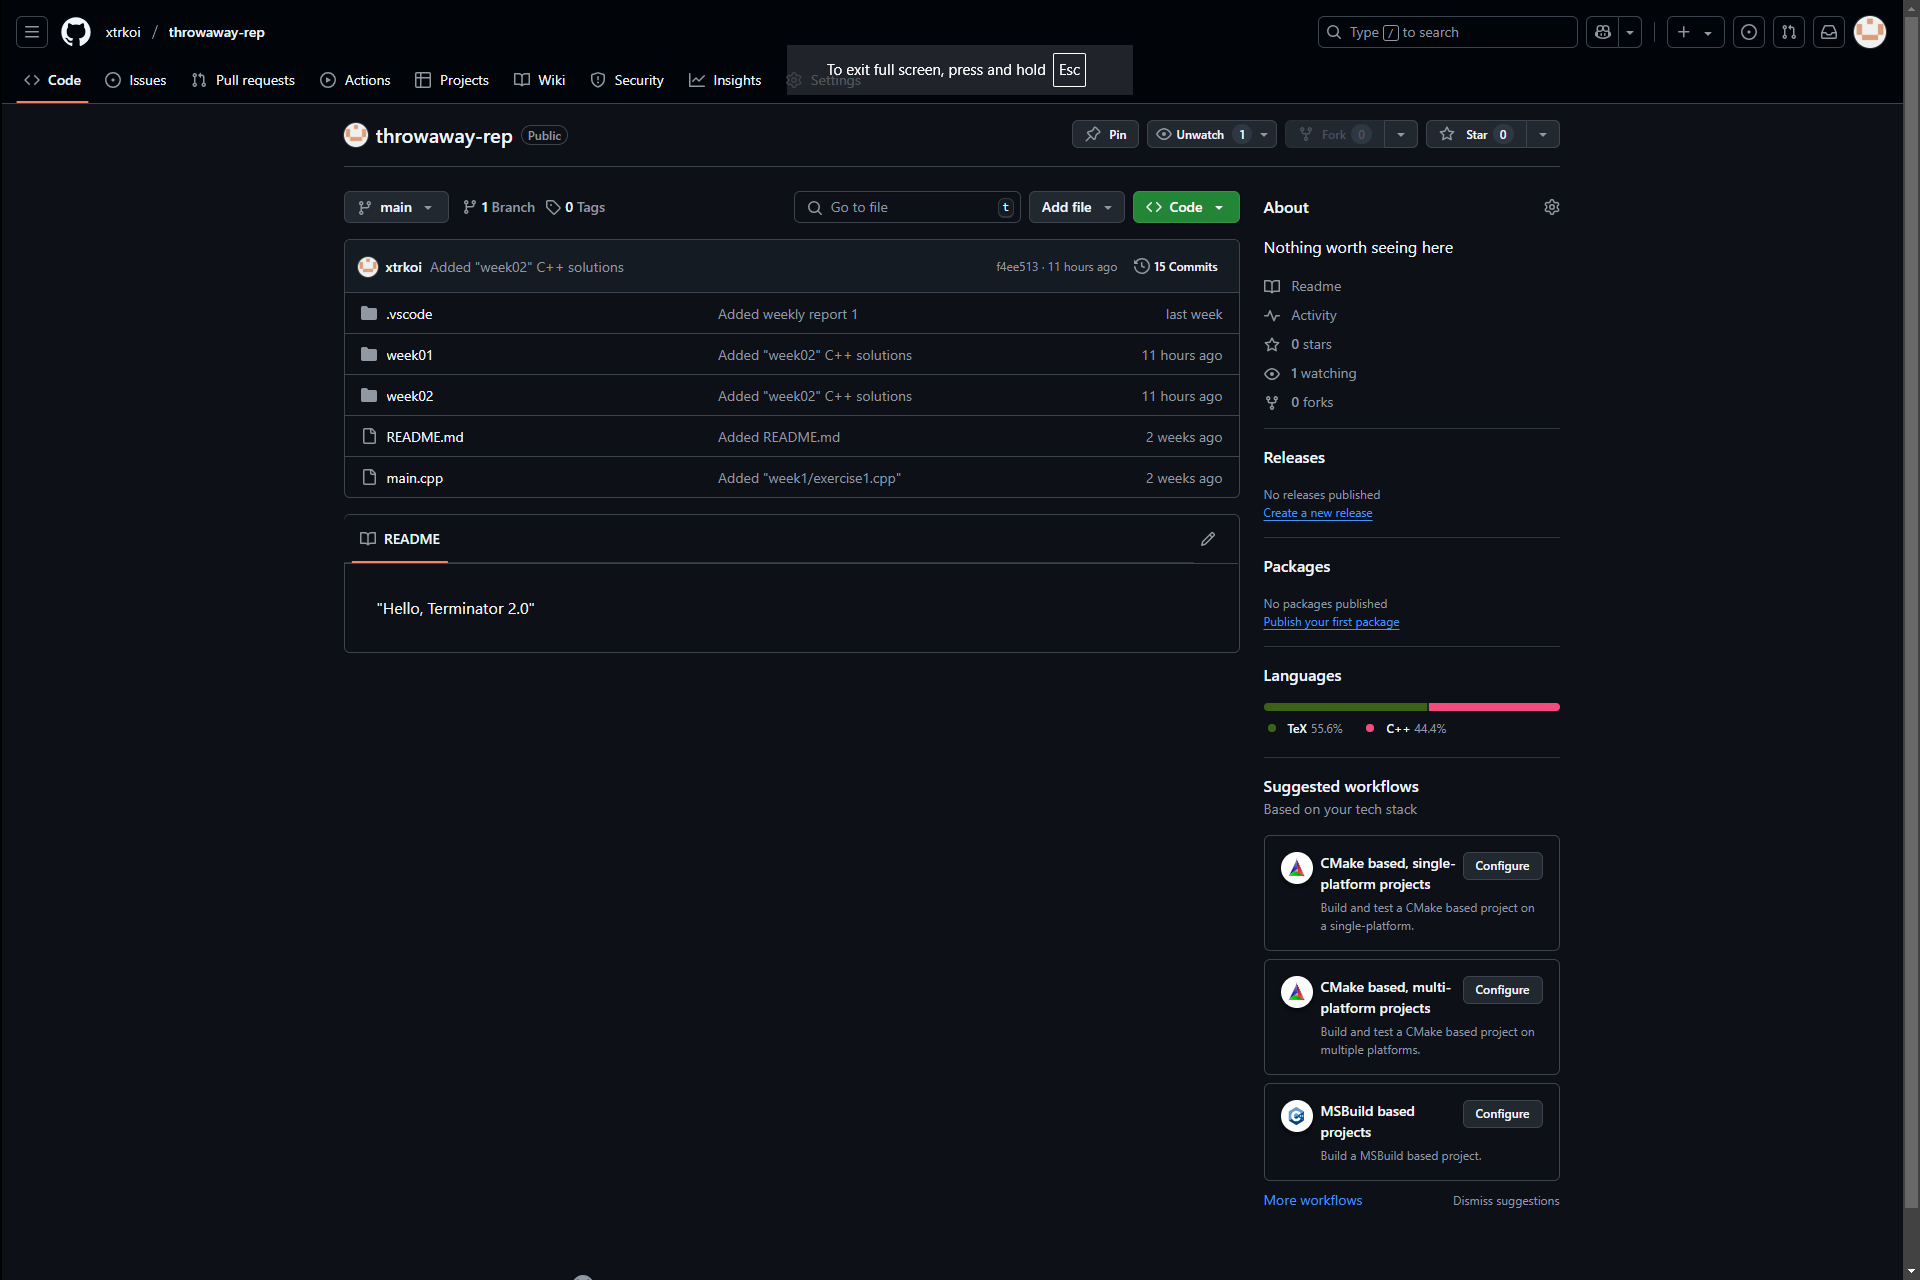
\includegraphics[width=12cm]{figure01.png}\hfil
        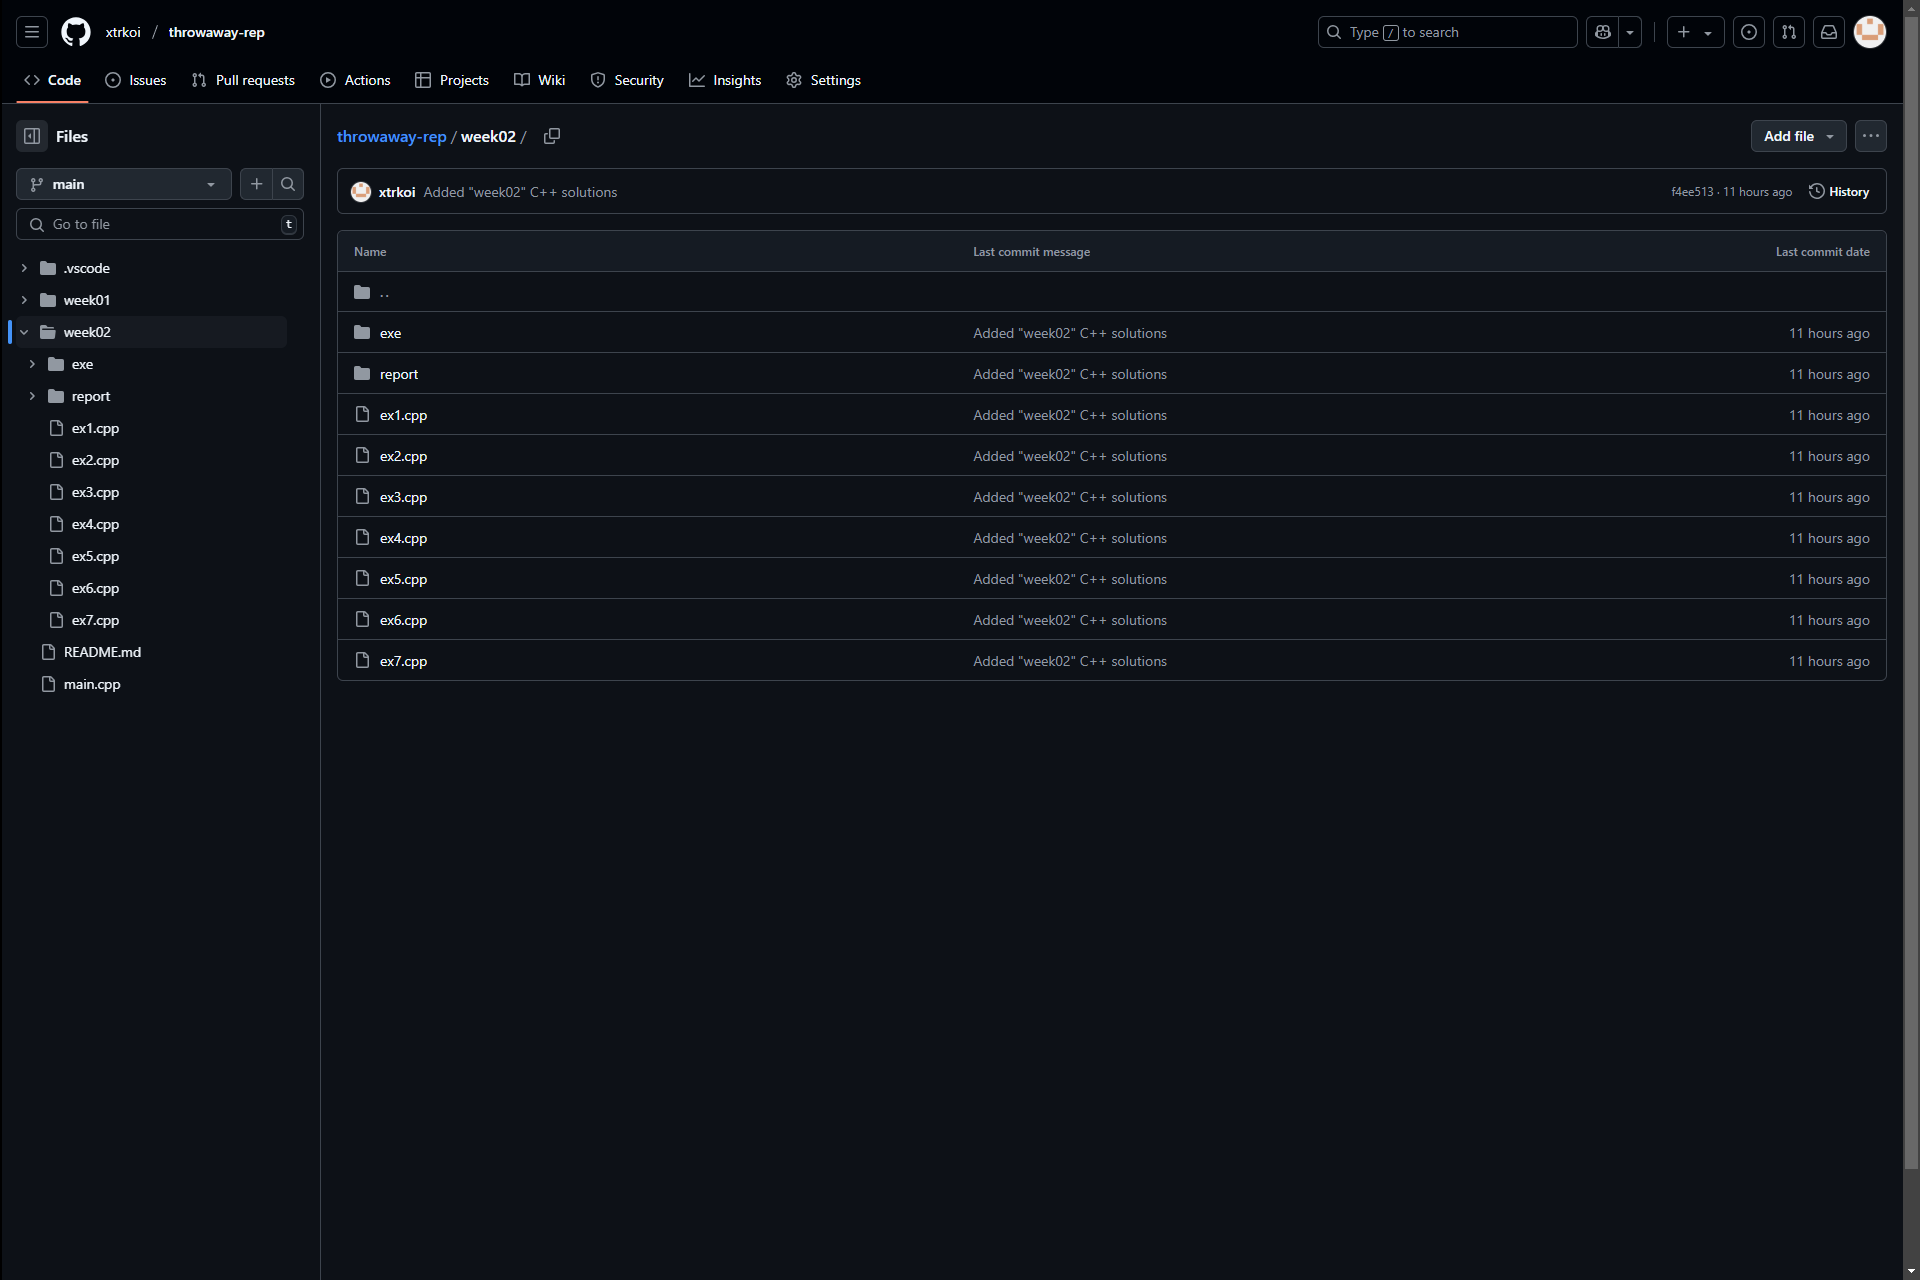
\includegraphics[width=12cm]{figure02.png}
        \caption{Online Github Repository}
    \end{figure}

    \section{The Problems}

    \subsection{Linear Search}

    \begin{statement}{Linear Search}{}
        Given an array of $N$ integers and a target integer $K$, implement a function to find the first occurence of $K$ in the array using Linear Search. If $K$ is found, return its (0-based) index. Otherwise, return $-1$.
    \end{statement}
    \label{linear-search}

    \emph{Approach.} Iterate from left to right to find the first occurence, right to left to find the last. Runs in $O(n)$.


    \subsection{Linear Search with Sentinel}

    \begin{statement}{Linear Search with Sentinel}{}
        Solve Problem \ref{linear-search} using Linear Search with Sentinel.
    \end{statement}

    \emph{Approach.} Set the last integer as the target integer to reduce out-of-range comparison checks.


    \subsection{Find the minimum element in a rotated array}

    \begin{statement}{}{}
        An array of length $n$, containing $n$ unique intgers, is sorted in ascending order, rotated between $1$ and $n$ times to the right. Find the minimum integer in the array.
    \end{statement}

    \emph{Approach.} Define $k$ as the last integer in the array ($a_{n - 1}$), and a function $\phi(x)$ which accepts any integer $x$ as input, and returns $0$ if $x > k$, $1$ if $x \le k$. It can be seen that $\phi(x)$ is monotonically increasing for $x \in \{a_0, a_1, \dots, a_{n - 1}\}$. We can use binary search to find the first $i$ so that $\phi(x) = \phi(a_i) = 1$. The answer is $a_i$ and the program runs in $O(\log n)$ as only binary search is used.


    \subsection{Find the minimum capacity}

    \begin{statement}{}{}
        There are $n$ packages ready to be shiped in order, the \emph{i-th} package has weight $w_i$. The ship has a capacity $C$ and can carry packages with the sum of weights not exceeding $C$ in any given day. The ship also has only $D$ days to ship the packages. Find the minimal $C$ that satisfy.
    \end{statement}

    \emph{Approach.} Define $\phi(x)$ as a function that returns $1$ if all packages can be delivered in $x$ days, $0$ otherwise. It can be proved that if there exists $a$ so $\phi(a) = 1$, then $\phi(x) = 1 \forall x \ge a$ and $\phi(x) = 0 \forall x < a$. This shows $\phi(x)$ is monotonically increasing, and by applying binary search, we can find the value $a$.

    Since the order of the packages are given, $\phi(x)$ can be implemented by load the maximum possible number of packages in any given day, then compare the number of days needed to deliver all packages to $x$.


    \subsection{Shortest subarray with at least given sum}

    \begin{statement}{}{}
        An array of $n$ positive integers is given, along with a target sum $T$. Find the length of the shortest subarray $[a_L, a_{L+1}, \dots, a_R]$ that has the sum $\sum_{i=L}^{R} a_i$ greater than or equal to $T$.
    \end{statement}

    \emph{Approach.} Define a partial sum array $[P_i] = [\sum_{j=0}^{i} a_i]$ for $i \in [0, n)$. Since $a_i > 0 \forall i \in [0, n)$, $[P_i]$ is monotonically increasing. The sum $\sum_{i=L}^{R} a_i$ can be calculated as

    \begin{equation*}
        \begin{cases}
            P_R, &\text{if} \quad L = 0 \\
            P_R - P_{L-1}, &\text{if} \quad L > 0
        \end{cases}
    \end{equation*}

    By iterating $L$, this problem can be converted into finding a value $k = T - P_{L-1}$ or $k = T$ if $L = 0$ in a sorted array with binary search, which runs in $O(n \log n)$.


    \subsection{Find a pair with given sum}

    \begin{statement}{}{}
        Given a sorted array of $n$ integers and a target sum $T$, determine if there exists $i, j \in [0, n); i \ne j$ so $a_i + a_j = T$.
    \end{statement}

    \emph{Approach.} Iterate $i$ and find $T - a_i$ with binary search.


    \subsection{Find all zero-sum triplets}

    \begin{statement}{}{}
        Given an array $a$ of $n$ integers, find all distinct triplets $\{a_i, a_j, a_k\}, i \ne j \ne k$ so that $a_i + a_j + a_k = 0$. The triplets can be output in any order.
    \end{statement}

    \emph{Approach.}

   
    \section{Conclusion}

    
    

\end{document}